\section{Sparse LOSS witnesses}
\label{sec:witnesses}

A LOSS leaf names current attacker threats whose empty sets cannot all be hit
within the defender's remaining budget.  Naming the complete threat family is
unnecessary.  The special geometry of six-cell Hexo windows gives smaller
witness families than a general rank-two hypergraph.

\begin{lemma}[Hexo-sparse LOSS witnesses]
\label{lem:L13}
A \cref{def:D9} LOSS witness can be chosen with at most three windows when
$b=1$ and at most five windows when $b=2$.  Both bounds are sharp among Hexo
threat-window families.
\end{lemma}

\begin{proof}
Every threat empty set has size one or two.

Suppose first that $b=1$.  If the family contains a singleton $\{a\}$, choose
that set and one member missing $a$.  Such a member exists because the full
family has transversal number greater than one.  If there is no singleton,
start with a pair $\{a,b\}$.  Choose one member missing $a$ and one member
missing $b$.  No single cell hits the selected family.  At most three members
are used.

Now let $b=2$.  If the family contains a singleton $\{a\}$, let
$\mathcal H$ be the subfamily of members missing $a$.  If
$\tau(\mathcal H)\le1$, then $a$ together with a one-point transversal of
$\mathcal H$ would hit the full family.  Hence $\tau(\mathcal H)>1$.  The
$b=1$ argument selects at most three members of $\mathcal H$; adjoining
$\{a\}$ uses at most four, and therefore at most five.

It remains to consider a family of pairs.  Choose an inclusion-minimal
subfamily $\mathcal G$ with $\tau(\mathcal G)>2$.  A general rank-two
selection uses at most six members.  To see this, take a maximal disjoint
subfamily.  Three disjoint pairs already have transversal number three.  One
pair cannot be maximal, because its two endpoints would then hit every
member.  In the remaining case take two disjoint members
\[
E_1=\{a,b\},\qquad E_2=\{c,d\}.
\]
Their four two-point transversals are
$\{a,c\},\{a,d\},\{b,c\},\{b,d\}$.  For each cross-pair, choose one member of
$\mathcal G$ that it misses.  Together with $E_1,E_2$, these choices use at
most six members and exclude every two-point transversal.

Assume equality six is necessary.  The four missing members must be distinct,
and each must miss only its assigned cross-pair.  A two-set missing
$\{a,c\}$ while meeting the other three cross-pairs must be $\{b,d\}$.
Using only one of $b,d$ would miss another cross-pair, while using two outside
points would be disjoint from both $E_1$ and $E_2$.  Cycling this argument
gives $\{b,c\}$, $\{a,d\}$, and $\{a,c\}$.  Thus a six-member minimal
obstruction is exactly the six edges of $K_4$.

Such a $K_4$ cannot be a Hexo threat-empty family.  Each empty pair lies on
one grid axis by \cref{fact:F1}.  To classify four pairwise axis-collinear
cells, translate one of them to the origin.  If the other three use the three
different incident axes, write them as
\[
 (u,0),\qquad(0,v),\qquad(w,-w),
\]
with $u,v,w\ne0$.  Pairwise axis alignment forces
$u=v=w=-v$, a contradiction.  If two of the other cells use the same axis,
then three cells already lie on one common axis line.  An off-line fourth cell
has only two nonparallel axis lines through it that meet this common line, so
it cannot align with all three distinct cells.  Hence all four lie on one
common axis line.  Order them $p_1<p_2<p_3<p_4$.  Any consecutive six-cell
window containing $p_1$ and $p_3$ also contains the intervening empty $p_2$.
Its empty set cannot be the $K_4$ edge $\{p_1,p_3\}$.  This is a
contradiction, so $|\mathcal G|\le5$.

The two constructions below attain three and five, respectively.  They show
sharpness among Hexo threat-window families.
\end{proof}

\begin{plainterms}
A verifier never needs a large collection of LOSS windows.  Three named
windows suffice with one defender placement left, and five suffice with two.
The five-window bound uses Hexo line geometry; a general family of pairs can
need the six edges of $K_4$.
\end{plainterms}

\subsection{The sharp three-window configuration}

Let
\[
a=(4,0),\qquad b=(5,0),\qquad c=(4,1),
\]
and define
\[
\begin{aligned}
W_{ab}&=\{(i,0):0\le i\le5\},\\
W_{ac}&=\{(4,i):-4\le i\le1\},\\
W_{bc}&=\{(5-i,i):0\le i\le5\}.
\end{aligned}
\]
Place attacker stones on
$(W_{ab}\cup W_{ac}\cup W_{bc})\setminus\{a,b,c\}$ and defender blockers at
\[
(-1,0),\qquad(4,-5),\qquad(-1,6).
\]
The origin is an attacker stone.  Exhaustive window enumeration gives exactly
three attacker threats, with empty sets
\[
\{a,b\},\qquad\{a,c\},\qquad\{b,c\}.
\]
Their transversal number is two.  Every subfamily of at most two has a common
point, so all three windows are required at a $b=1$ LOSS leaf.  After any one
defender placement, one edge remains untouched and the attacker fills its two
cells.

\begin{figure}[tbp]
  \centering
  \begin{tikzpicture}[scale=.38]
    \HexPatch{-1/0,4/-5,-1/6,
      0/0,1/0,2/0,3/0,4/0,5/0,
      4/-4,4/-3,4/-2,4/-1,4/1,
      3/2,2/3,1/4,0/5}
    \HexWindow[fill=black!9,draw=none]{0}{0}{1}{0}
    \HexWindow[fill=black!19,draw=none]{4}{-4}{0}{1}
    \HexWindow[fill=none,draw=black,dashed,line width=1pt]{5}{0}{-1}{1}
    \HexAttackerList{0/0,1/0,2/0,3/0,
      4/-4,4/-3,4/-2,4/-1,3/2,2/3,1/4,0/5}
    \HexDefenderList{-1/0,4/-5,-1/6}
    \HexCellText{4}{0}{$a$}
    \HexCellText{5}{0}{$b$}
    \HexCellText{4}{1}{$c$}
  \end{tikzpicture}
  \caption{The triangle witness for $b=1$.  The three labelled empty cells
  give the three pair edges; the open disks are the blockers that remove
  shifted threats.}
  \label{fig:witness-triangle}
\end{figure}

\subsection{The sharp five-window configuration}

Let
\[
v_0=(4,0),\quad v_1=(5,0),\quad v_2=(6,0),\quad
v_3=(4,2),\quad v_4=(4,1).
\]
Use the five windows
\[
\begin{array}{c@{\qquad}c}
W_{01}=\{(i,0):0\le i\le5\},&
W_{12}=\{(5+i,0):0\le i\le5\},\\
W_{23}=\{(6-i,i):0\le i\le5\},&
W_{34}=\{(4,1+i):0\le i\le5\},\\
\multicolumn{2}{c}{W_{40}=\{(4,-4+i):0\le i\le5\}.}
\end{array}
\]
Place attacker stones on their union minus the five vertices, and place
defender blockers at
\[
(-1,0),\quad(4,-5),\quad(11,0),\quad(4,7),\quad(0,6).
\]
The complete attacker-threat family is exactly
\[
\{v_0,v_1\},\ \{v_1,v_2\},\ \{v_2,v_3\},\
\ \{v_3,v_4\},\ \{v_4,v_0\}.
\]
It is the edge set of $C_5$.  Its vertex-cover number is three.  Removing any
edge leaves a four-edge path with vertex-cover number two.  Hence no four
windows have transversal number greater than two, while all five do.  The
finite checker enumerates twenty attacker stones, the five blockers, every
incident window, the absence of a completion and of a defender immediate
win, and exactly these five threats.

\begin{figure}[tbp]
  \centering
  \begin{tikzpicture}[scale=.36]
    \HexPatch{-1/0,4/-5,11/0,4/7,0/6,
      0/0,1/0,2/0,3/0,4/0,5/0,6/0,7/0,8/0,9/0,10/0,
      5/1,4/1,4/2,3/3,2/4,1/5,
      4/3,4/4,4/5,4/6,
      4/-4,4/-3,4/-2,4/-1}
    \HexWindow[fill=black!6,draw=none]{0}{0}{1}{0}
    \HexWindow[fill=black!12,draw=none]{5}{0}{1}{0}
    \HexWindow[fill=black!18,draw=none]{6}{0}{-1}{1}
    \HexWindow[fill=black!24,draw=none]{4}{1}{0}{1}
    \HexWindow[fill=none,draw=black,dashed,line width=1pt]{4}{-4}{0}{1}
    \HexAttackerList{0/0,1/0,2/0,3/0,7/0,8/0,9/0,10/0,
      5/1,3/3,2/4,1/5,4/3,4/4,4/5,4/6,
      4/-4,4/-3,4/-2,4/-1}
    \HexDefenderList{-1/0,4/-5,11/0,4/7,0/6}
    \HexCellText{4}{0}{$v_0$}
    \HexCellText{5}{0}{$v_1$}
    \HexCellText{6}{0}{$v_2$}
    \HexCellText{4}{2}{$v_3$}
    \HexCellText{4}{1}{$v_4$}
  \end{tikzpicture}
  \caption{The five-cycle witness for $b=2$.  Each shaded or outlined window
  has one adjacent pair of labelled empties.}
  \label{fig:witness-cycle}
\end{figure}

The caps are relative to the named-window LOSS format.  A smaller cap would
reject the displayed valid leaves.  The constructions do not rule out a
different terminal representation with other witness data.
